\hypertarget{t__hashtab_8c}{
\section{t\_\-hashtab.c File Reference}
\label{t__hashtab_8c}\index{t_hashtab.c@{t\_\-hashtab.c}}
}


{\tt \#include $<$stdio.h$>$}\par
{\tt \#include $<$stdlib.h$>$}\par
{\tt \#include $<$string.h$>$}\par
{\tt \#include $<$time.h$>$}\par
{\tt \#include \char`\"{}test-harness.h\char`\"{}}\par
{\tt \#include \char`\"{}dbprim.h\char`\"{}}\par
{\tt \#include \char`\"{}dbprim\_\-int.h\char`\"{}}\par


Include dependency graph for t\_\-hashtab.c:\begin{figure}[H]
\begin{center}
\leavevmode
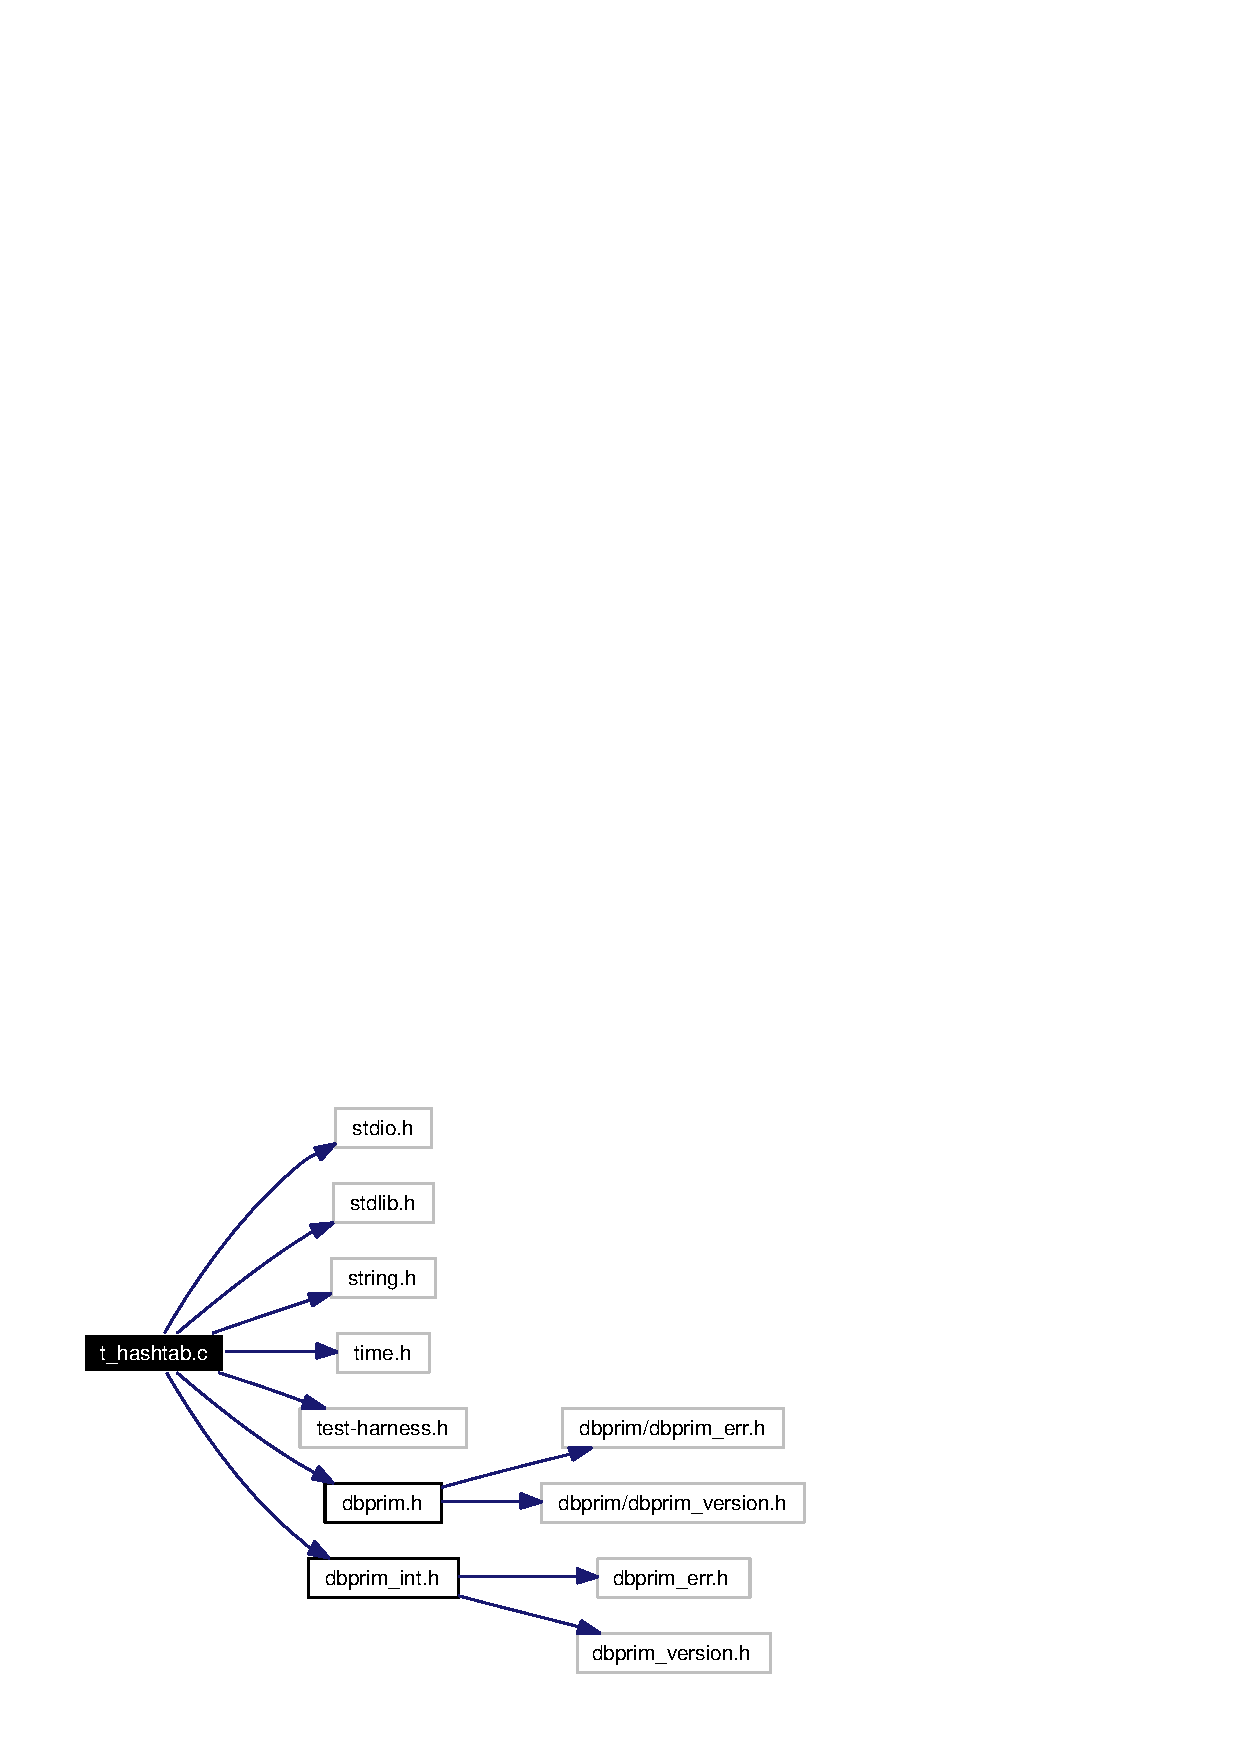
\includegraphics[width=195pt]{t__hashtab_8c__incl}
\end{center}
\end{figure}
\subsection*{Data Structures}
\begin{CompactItemize}
\item 
struct \hyperlink{structmoves__s}{moves\_\-s}
\item 
struct \hyperlink{structiter__s}{iter\_\-s}
\end{CompactItemize}
\subsection*{Defines}
\begin{CompactItemize}
\item 
\#define \hyperlink{t__hashtab_8c_a0}{FLUSH\_\-THRESHOLD}
\item 
\#define \hyperlink{t__hashtab_8c_a1}{\_\-hw}(n, m, s)
\item 
\#define \hyperlink{t__hashtab_8c_a2}{RSF\_\-INHIBIT}
\item 
\#define \hyperlink{t__hashtab_8c_a3}{RSF\_\-RESIZE}
\item 
\#define \hyperlink{t__hashtab_8c_a4}{HASH\_\-ENT\_\-CNT}
\item 
\#define \hyperlink{t__hashtab_8c_a5}{HASH\_\-MOVE\_\-CNT}
\item 
\#define \hyperlink{t__hashtab_8c_a6}{HASH\_\-REMOVE\_\-CNT}
\item 
\#define \hyperlink{t__hashtab_8c_a7}{VISIT\_\-INIT}
\end{CompactItemize}
\subsection*{Functions}
\begin{CompactItemize}
\item 
static unsigned long \hyperlink{t__hashtab_8c_a14}{hamming} (unsigned long bits)
\item 
static unsigned long \hyperlink{t__hashtab_8c_a15}{t\_\-hash} (\hyperlink{struct__hash__table__s}{hash\_\-table\_\-t} $\ast$tab, \hyperlink{struct__db__key__s}{db\_\-key\_\-t} $\ast$key)
\item 
static unsigned long \hyperlink{t__hashtab_8c_a16}{t\_\-comp} (\hyperlink{struct__hash__table__s}{hash\_\-table\_\-t} $\ast$tab, \hyperlink{struct__db__key__s}{db\_\-key\_\-t} $\ast$key1, \hyperlink{struct__db__key__s}{db\_\-key\_\-t} $\ast$key2)
\item 
static unsigned long \hyperlink{t__hashtab_8c_a17}{t\_\-resize} (\hyperlink{struct__hash__table__s}{hash\_\-table\_\-t} $\ast$tab, unsigned long new)
\item 
static unsigned long \hyperlink{t__hashtab_8c_a18}{t\_\-iter} (\hyperlink{struct__hash__table__s}{hash\_\-table\_\-t} $\ast$tab, \hyperlink{struct__hash__entry__s}{hash\_\-entry\_\-t} $\ast$ent, struct \hyperlink{structiter__s}{iter\_\-s} $\ast$iter)
\item 
int \hyperlink{t__hashtab_8c_a19}{main} (int argc, char $\ast$$\ast$argv)
\end{CompactItemize}
\subsection*{Variables}
\begin{CompactItemize}
\item 
static unsigned int \hyperlink{t__hashtab_8c_a8}{rsize\_\-flags}
\item 
static unsigned long \hyperlink{t__hashtab_8c_a9}{rsize\_\-new}
\item 
static unsigned long \hyperlink{t__hashtab_8c_a10}{rsize\_\-err}
\item 
static \hyperlink{struct__db__key__s}{db\_\-key\_\-t} \hyperlink{t__hashtab_8c_a11}{keys} \mbox{[}$\,$\mbox{]}
\item 
static struct \hyperlink{structmoves__s}{moves\_\-s} \hyperlink{t__hashtab_8c_a12}{moves} \mbox{[}$\,$\mbox{]}
\item 
static int \hyperlink{t__hashtab_8c_a13}{removes} \mbox{[}$\,$\mbox{]}
\end{CompactItemize}


\subsection{Define Documentation}
\hypertarget{t__hashtab_8c_a1}{
\index{t_hashtab.c@{t\_\-hashtab.c}!_hw@{\_\-hw}}
\index{_hw@{\_\-hw}!t_hashtab.c@{t\_\-hashtab.c}}
\subsubsection[\_\-hw]{\setlength{\rightskip}{0pt plus 5cm}\#define \_\-hw(n, m, s)}}
\label{t__hashtab_8c_a1}




Referenced by hamming().\hypertarget{t__hashtab_8c_a0}{
\index{t_hashtab.c@{t\_\-hashtab.c}!FLUSH_THRESHOLD@{FLUSH\_\-THRESHOLD}}
\index{FLUSH_THRESHOLD@{FLUSH\_\-THRESHOLD}!t_hashtab.c@{t\_\-hashtab.c}}
\subsubsection[FLUSH\_\-THRESHOLD]{\setlength{\rightskip}{0pt plus 5cm}\#define FLUSH\_\-THRESHOLD}}
\label{t__hashtab_8c_a0}




Definition at line 35 of file t\_\-hashtab.c.

Referenced by main().\hypertarget{t__hashtab_8c_a4}{
\index{t_hashtab.c@{t\_\-hashtab.c}!HASH_ENT_CNT@{HASH\_\-ENT\_\-CNT}}
\index{HASH_ENT_CNT@{HASH\_\-ENT\_\-CNT}!t_hashtab.c@{t\_\-hashtab.c}}
\subsubsection[HASH\_\-ENT\_\-CNT]{\setlength{\rightskip}{0pt plus 5cm}\#define HASH\_\-ENT\_\-CNT}}
\label{t__hashtab_8c_a4}




Definition at line 121 of file t\_\-hashtab.c.

Referenced by main().\hypertarget{t__hashtab_8c_a5}{
\index{t_hashtab.c@{t\_\-hashtab.c}!HASH_MOVE_CNT@{HASH\_\-MOVE\_\-CNT}}
\index{HASH_MOVE_CNT@{HASH\_\-MOVE\_\-CNT}!t_hashtab.c@{t\_\-hashtab.c}}
\subsubsection[HASH\_\-MOVE\_\-CNT]{\setlength{\rightskip}{0pt plus 5cm}\#define HASH\_\-MOVE\_\-CNT}}
\label{t__hashtab_8c_a5}




Definition at line 139 of file t\_\-hashtab.c.

Referenced by main().\hypertarget{t__hashtab_8c_a6}{
\index{t_hashtab.c@{t\_\-hashtab.c}!HASH_REMOVE_CNT@{HASH\_\-REMOVE\_\-CNT}}
\index{HASH_REMOVE_CNT@{HASH\_\-REMOVE\_\-CNT}!t_hashtab.c@{t\_\-hashtab.c}}
\subsubsection[HASH\_\-REMOVE\_\-CNT]{\setlength{\rightskip}{0pt plus 5cm}\#define HASH\_\-REMOVE\_\-CNT}}
\label{t__hashtab_8c_a6}




Definition at line 143 of file t\_\-hashtab.c.

Referenced by main().\hypertarget{t__hashtab_8c_a2}{
\index{t_hashtab.c@{t\_\-hashtab.c}!RSF_INHIBIT@{RSF\_\-INHIBIT}}
\index{RSF_INHIBIT@{RSF\_\-INHIBIT}!t_hashtab.c@{t\_\-hashtab.c}}
\subsubsection[RSF\_\-INHIBIT]{\setlength{\rightskip}{0pt plus 5cm}\#define RSF\_\-INHIBIT}}
\label{t__hashtab_8c_a2}




Definition at line 86 of file t\_\-hashtab.c.

Referenced by main(), and t\_\-resize().\hypertarget{t__hashtab_8c_a3}{
\index{t_hashtab.c@{t\_\-hashtab.c}!RSF_RESIZE@{RSF\_\-RESIZE}}
\index{RSF_RESIZE@{RSF\_\-RESIZE}!t_hashtab.c@{t\_\-hashtab.c}}
\subsubsection[RSF\_\-RESIZE]{\setlength{\rightskip}{0pt plus 5cm}\#define RSF\_\-RESIZE}}
\label{t__hashtab_8c_a3}




Definition at line 87 of file t\_\-hashtab.c.

Referenced by main(), and t\_\-resize().\hypertarget{t__hashtab_8c_a7}{
\index{t_hashtab.c@{t\_\-hashtab.c}!VISIT_INIT@{VISIT\_\-INIT}}
\index{VISIT_INIT@{VISIT\_\-INIT}!t_hashtab.c@{t\_\-hashtab.c}}
\subsubsection[VISIT\_\-INIT]{\setlength{\rightskip}{0pt plus 5cm}\#define VISIT\_\-INIT}}
\label{t__hashtab_8c_a7}




Definition at line 151 of file t\_\-hashtab.c.

Referenced by main().

\subsection{Function Documentation}
\hypertarget{t__hashtab_8c_a14}{
\index{t_hashtab.c@{t\_\-hashtab.c}!hamming@{hamming}}
\index{hamming@{hamming}!t_hashtab.c@{t\_\-hashtab.c}}
\subsubsection[hamming]{\setlength{\rightskip}{0pt plus 5cm}static unsigned long hamming (unsigned long {\em bits})\hspace{0.3cm}{\tt  \mbox{[}static\mbox{]}}}}
\label{t__hashtab_8c_a14}




Definition at line 39 of file t\_\-hashtab.c.

References \_\-hw.

Referenced by main().\hypertarget{t__hashtab_8c_a19}{
\index{t_hashtab.c@{t\_\-hashtab.c}!main@{main}}
\index{main@{main}!t_hashtab.c@{t\_\-hashtab.c}}
\subsubsection[main]{\setlength{\rightskip}{0pt plus 5cm}int main (int {\em argc}, char $\ast$$\ast$ {\em argv})}}
\label{t__hashtab_8c_a19}




Definition at line 170 of file t\_\-hashtab.c.

References iter\_\-s::elem, FLUSH\_\-THRESHOLD, hamming(), HASH\_\-ENT\_\-CNT, HASH\_\-FLAG\_\-AUTOGROW, HASH\_\-FLAG\_\-AUTOSHRINK, HASH\_\-MOVE\_\-CNT, HASH\_\-REMOVE\_\-CNT, he\_\-init(), ht\_\-add(), ht\_\-count, ht\_\-find(), ht\_\-flags, ht\_\-flush(), ht\_\-free(), ht\_\-init(), ht\_\-iter(), ht\_\-modulus, ht\_\-move(), ht\_\-remove(), ht\_\-resize(), \_\-hash\_\-table\_\-s::ht\_\-table, moves, removes, RSF\_\-INHIBIT, RSF\_\-RESIZE, rsize\_\-err, rsize\_\-flags, rsize\_\-new, t\_\-comp(), t\_\-hash(), t\_\-iter(), t\_\-resize(), VISIT\_\-INIT, and iter\_\-s::visited.

Here is the call graph for this function:\begin{figure}[H]
\begin{center}
\leavevmode
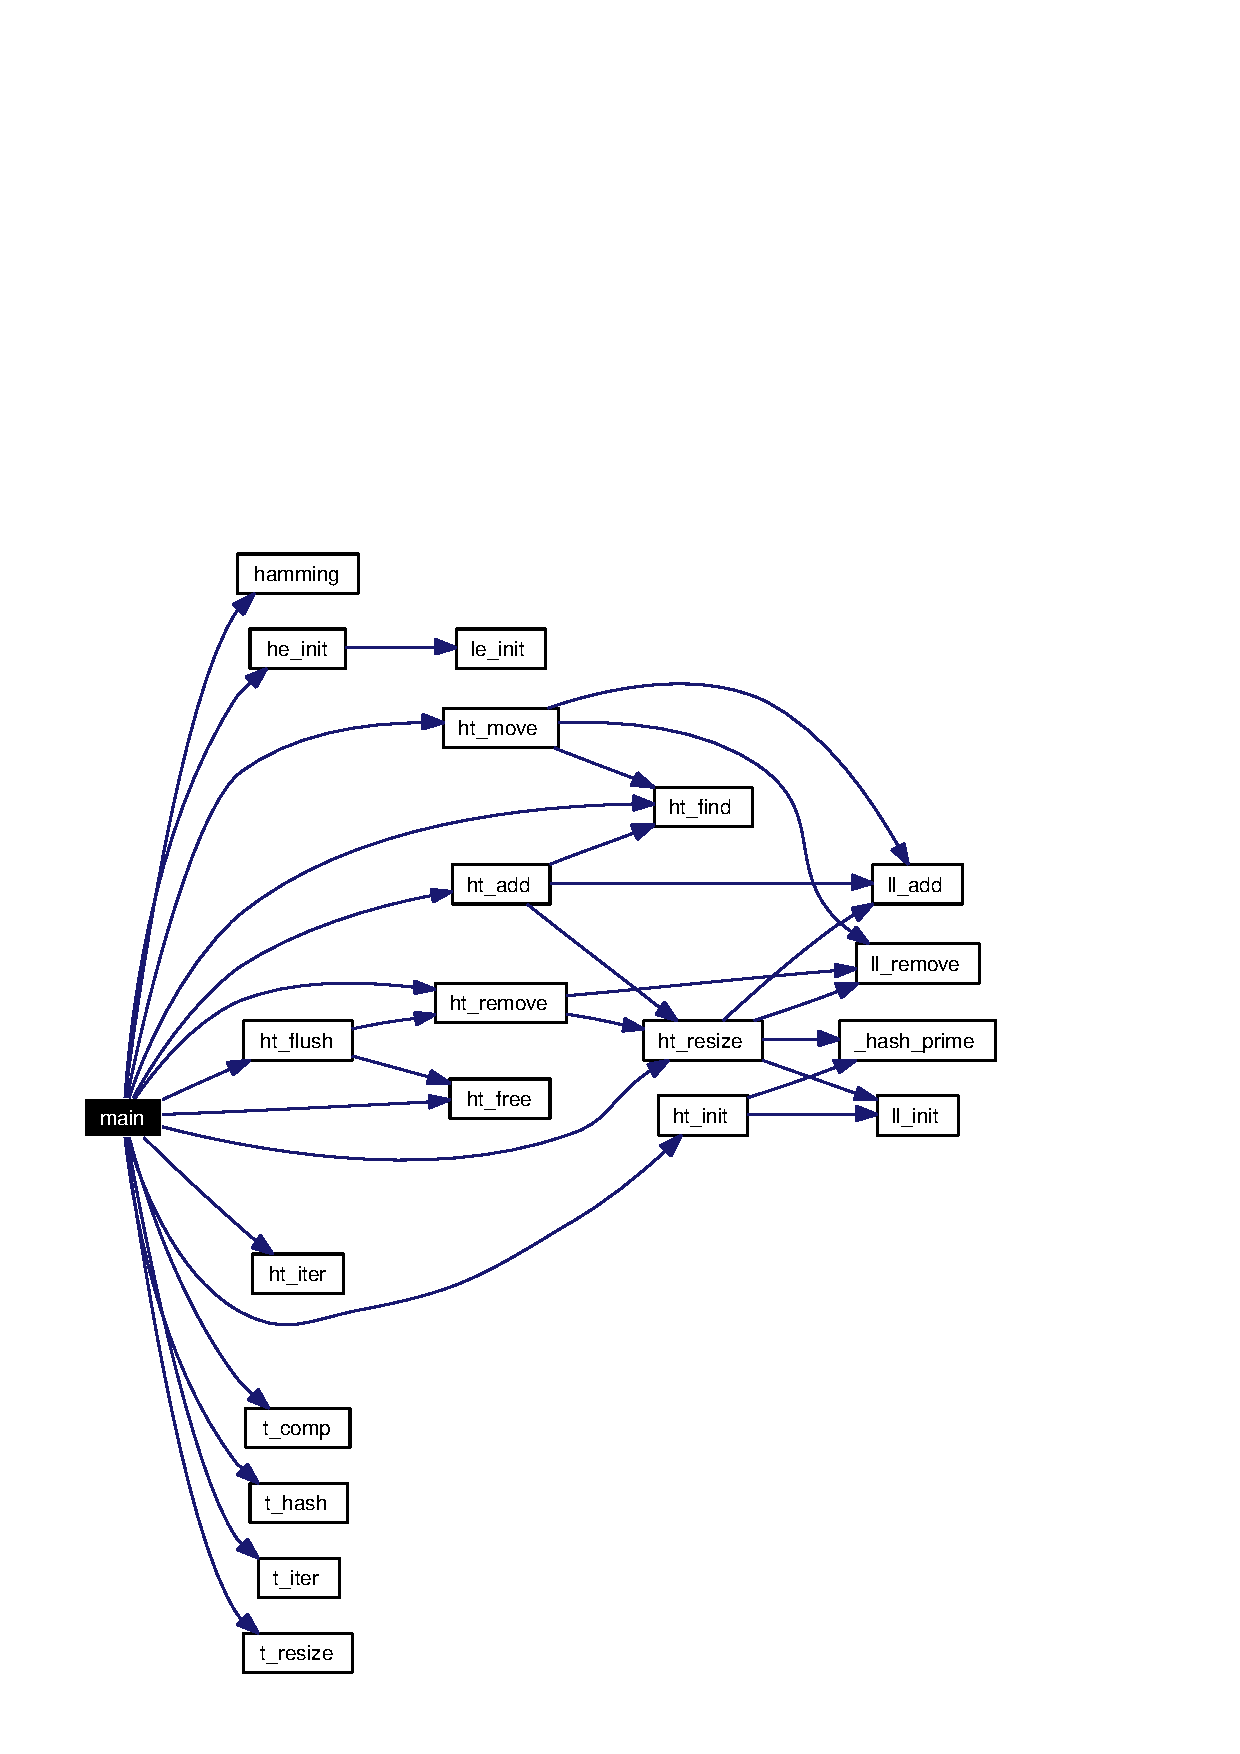
\includegraphics[width=241pt]{t__hashtab_8c_a19_cgraph}
\end{center}
\end{figure}
\hypertarget{t__hashtab_8c_a16}{
\index{t_hashtab.c@{t\_\-hashtab.c}!t_comp@{t\_\-comp}}
\index{t_comp@{t\_\-comp}!t_hashtab.c@{t\_\-hashtab.c}}
\subsubsection[t\_\-comp]{\setlength{\rightskip}{0pt plus 5cm}static unsigned long t\_\-comp (\hyperlink{struct__hash__table__s}{hash\_\-table\_\-t} $\ast$ {\em tab}, \hyperlink{struct__db__key__s}{db\_\-key\_\-t} $\ast$ {\em key1}, \hyperlink{struct__db__key__s}{db\_\-key\_\-t} $\ast$ {\em key2})\hspace{0.3cm}{\tt  \mbox{[}static\mbox{]}}}}
\label{t__hashtab_8c_a16}




Definition at line 70 of file t\_\-hashtab.c.

References dk\_\-key, and dk\_\-len.

Referenced by main().\hypertarget{t__hashtab_8c_a15}{
\index{t_hashtab.c@{t\_\-hashtab.c}!t_hash@{t\_\-hash}}
\index{t_hash@{t\_\-hash}!t_hashtab.c@{t\_\-hashtab.c}}
\subsubsection[t\_\-hash]{\setlength{\rightskip}{0pt plus 5cm}static unsigned long t\_\-hash (\hyperlink{struct__hash__table__s}{hash\_\-table\_\-t} $\ast$ {\em tab}, \hyperlink{struct__db__key__s}{db\_\-key\_\-t} $\ast$ {\em key})\hspace{0.3cm}{\tt  \mbox{[}static\mbox{]}}}}
\label{t__hashtab_8c_a15}




Definition at line 53 of file t\_\-hashtab.c.

References dk\_\-key, and dk\_\-len.

Referenced by main().\hypertarget{t__hashtab_8c_a18}{
\index{t_hashtab.c@{t\_\-hashtab.c}!t_iter@{t\_\-iter}}
\index{t_iter@{t\_\-iter}!t_hashtab.c@{t\_\-hashtab.c}}
\subsubsection[t\_\-iter]{\setlength{\rightskip}{0pt plus 5cm}static unsigned long t\_\-iter (\hyperlink{struct__hash__table__s}{hash\_\-table\_\-t} $\ast$ {\em tab}, \hyperlink{struct__hash__entry__s}{hash\_\-entry\_\-t} $\ast$ {\em ent}, struct \hyperlink{structiter__s}{iter\_\-s} $\ast$ {\em iter})\hspace{0.3cm}{\tt  \mbox{[}static\mbox{]}}}}
\label{t__hashtab_8c_a18}




Definition at line 154 of file t\_\-hashtab.c.

References iter\_\-s::elem, iter\_\-s::err, he\_\-value, and iter\_\-s::visited.

Referenced by main().\hypertarget{t__hashtab_8c_a17}{
\index{t_hashtab.c@{t\_\-hashtab.c}!t_resize@{t\_\-resize}}
\index{t_resize@{t\_\-resize}!t_hashtab.c@{t\_\-hashtab.c}}
\subsubsection[t\_\-resize]{\setlength{\rightskip}{0pt plus 5cm}static unsigned long t\_\-resize (\hyperlink{struct__hash__table__s}{hash\_\-table\_\-t} $\ast$ {\em tab}, unsigned long {\em new})\hspace{0.3cm}{\tt  \mbox{[}static\mbox{]}}}}
\label{t__hashtab_8c_a17}




Definition at line 94 of file t\_\-hashtab.c.

References RSF\_\-INHIBIT, RSF\_\-RESIZE, rsize\_\-err, rsize\_\-flags, and rsize\_\-new.

Referenced by main().

\subsection{Variable Documentation}
\hypertarget{t__hashtab_8c_a11}{
\index{t_hashtab.c@{t\_\-hashtab.c}!keys@{keys}}
\index{keys@{keys}!t_hashtab.c@{t\_\-hashtab.c}}
\subsubsection[keys]{\setlength{\rightskip}{0pt plus 5cm}\hyperlink{struct__db__key__s}{db\_\-key\_\-t} \hyperlink{t__hashtab_8c_a11}{keys}\mbox{[}$\,$\mbox{]}\hspace{0.3cm}{\tt  \mbox{[}static\mbox{]}}}}
\label{t__hashtab_8c_a11}




Definition at line 103 of file t\_\-hashtab.c.\hypertarget{t__hashtab_8c_a12}{
\index{t_hashtab.c@{t\_\-hashtab.c}!moves@{moves}}
\index{moves@{moves}!t_hashtab.c@{t\_\-hashtab.c}}
\subsubsection[moves]{\setlength{\rightskip}{0pt plus 5cm}struct \hyperlink{structmoves__s}{moves\_\-s}  \hyperlink{t__hashtab_8c_a12}{moves}\mbox{[}$\,$\mbox{]}\hspace{0.3cm}{\tt  \mbox{[}static\mbox{]}}}}
\label{t__hashtab_8c_a12}




Referenced by main().\hypertarget{t__hashtab_8c_a13}{
\index{t_hashtab.c@{t\_\-hashtab.c}!removes@{removes}}
\index{removes@{removes}!t_hashtab.c@{t\_\-hashtab.c}}
\subsubsection[removes]{\setlength{\rightskip}{0pt plus 5cm}int \hyperlink{t__hashtab_8c_a13}{removes}\mbox{[}$\,$\mbox{]}\hspace{0.3cm}{\tt  \mbox{[}static\mbox{]}}}}
\label{t__hashtab_8c_a13}




Definition at line 141 of file t\_\-hashtab.c.

Referenced by main().\hypertarget{t__hashtab_8c_a10}{
\index{t_hashtab.c@{t\_\-hashtab.c}!rsize_err@{rsize\_\-err}}
\index{rsize_err@{rsize\_\-err}!t_hashtab.c@{t\_\-hashtab.c}}
\subsubsection[rsize\_\-err]{\setlength{\rightskip}{0pt plus 5cm}unsigned long \hyperlink{t__hashtab_8c_a10}{rsize\_\-err}\hspace{0.3cm}{\tt  \mbox{[}static\mbox{]}}}}
\label{t__hashtab_8c_a10}




Definition at line 90 of file t\_\-hashtab.c.

Referenced by main(), and t\_\-resize().\hypertarget{t__hashtab_8c_a8}{
\index{t_hashtab.c@{t\_\-hashtab.c}!rsize_flags@{rsize\_\-flags}}
\index{rsize_flags@{rsize\_\-flags}!t_hashtab.c@{t\_\-hashtab.c}}
\subsubsection[rsize\_\-flags]{\setlength{\rightskip}{0pt plus 5cm}unsigned int \hyperlink{t__hashtab_8c_a8}{rsize\_\-flags}\hspace{0.3cm}{\tt  \mbox{[}static\mbox{]}}}}
\label{t__hashtab_8c_a8}




Definition at line 84 of file t\_\-hashtab.c.

Referenced by main(), and t\_\-resize().\hypertarget{t__hashtab_8c_a9}{
\index{t_hashtab.c@{t\_\-hashtab.c}!rsize_new@{rsize\_\-new}}
\index{rsize_new@{rsize\_\-new}!t_hashtab.c@{t\_\-hashtab.c}}
\subsubsection[rsize\_\-new]{\setlength{\rightskip}{0pt plus 5cm}unsigned long \hyperlink{t__hashtab_8c_a9}{rsize\_\-new}\hspace{0.3cm}{\tt  \mbox{[}static\mbox{]}}}}
\label{t__hashtab_8c_a9}




Definition at line 89 of file t\_\-hashtab.c.

Referenced by main(), and t\_\-resize().